% ==========================================
% BAB V IMPLEMENTASI
% ==========================================
\cleardoublepage
\chapter{IMPLEMENTASI SISTEM \textit{GRAPHRAG} BERBASIS \textit{KNOWLEDGE GRAPH} KUBERNETES}
\label{chap:implementasi}

% ─────────────────────────────────────────────────────────────────────
\section{Lingkungan Implementasi}
% ─────────────────────────────────────────────────────────────────────

Implementasi sistem \textit{GraphRAG} Kubernetes dilaksanakan menggunakan bahasa pemrograman Python 3.11 pada sistem operasi Windows 11. Seluruh dependensi dikelola melalui \textit{virtual environment} dan didefinisikan dalam berkas \texttt{requirements.txt}. Tabel~\ref{tbl:tech_stack} merangkum komponen utama beserta perannya dalam sistem.

\renewcommand{\arraystretch}{1.3}
\captionsetup[table]{justification=raggedright,singlelinecheck=false}
\begin{table}[H]
\caption{Dependensi Utama Implementasi Sistem GraphRAG Kubernetes}
\label{tbl:tech_stack}
\centering
\begin{tabular}{| p{0.25\textwidth} | p{0.15\textwidth} | p{0.47\textwidth} |}
\hline
\textbf{Komponen} & \textbf{Versi} & \textbf{Fungsi dalam Sistem} \\
\hline
LangGraph & 1.0.9 & Orkestrasi lima \textit{AI agent} berbasis \textit{state machine} (lihat Tabel~\ref{tbl:langgraph_nodes}) \\
\hline
LangChain-Core & 1.2.15 & Penyimpanan riwayat percakapan dalam sesi yang sama melalui format pesan \textit{BaseMessage}/\textit{AIMessage} \\
\hline
LangChain-OpenAI & 1.1.10 & \textit{ChatOpenAI} untuk node \textit{Thinker} (temp=0,0) dan \textit{Speaker} (temp=0,1); \textit{OpenAIEmbeddings} untuk evaluasi \\
\hline
Neo4j Python Driver & 6.1.0 & Koneksi dan eksekusi \textit{query} Cypher ke \textit{knowledge graph} \\
\hline
OpenAI SDK & 2.21.0 & Pembuatan \textit{embedding} \textit{text-embedding-3-small} \\
\hline
Streamlit & 1.54.0 & Antarmuka \textit{web} percakapan berbasis \textit{browser} \\
\hline
PyYAML & 6.0.3 & Validasi sintaksis YAML \\
\hline
kubernetes-validate & 1.35.0 & Validasi terhadap skema Kubernetes v1.29 \\
\hline
SQLite & \textit{stdlib} & Penyimpanan riwayat percakapan antarsesi \\
\hline
\end{tabular}
\end{table}


Sistem memanfaatkan \textbf{OpenAI GPT-4o-mini} untuk kedua peran LLM. \textit{Thinker} menggunakan GPT-4o-mini untuk mengekstraksi \textit{intent} kueri ke dalam format JSON terstruktur berkat kemampuan pemahaman konteks yang tinggi dan dukungan \textit{structured output}. \textit{Speaker} juga menggunakan GPT-4o-mini untuk menghasilkan respons naratif; penggunaan model yang sama dipilih guna memastikan konsistensi pemahaman skema Kubernetes antara tahap ekstraksi \textit{intent} dan tahap generasi jawaban.

Untuk penyimpanan percakapan, sistem menggunakan \textbf{SQLite} lokal yang diakses melalui kelas \textit{SQLiteMemoryStore} di \texttt{src/memory/zep\_store.py}. Keputusan ini diambil karena Zep Cloud versi 1 memanggil LLM internal untuk ekstraksi entitas yang menambah latensi dan biaya token tanpa nilai tambah bagi penelitian ini. SQLite memberikan persistensi yang memadai tanpa ketergantungan infrastruktur tambahan.

Antarmuka pengguna diimplementasikan menggunakan \textit{Streamlit} pada berkas \texttt{main.py} sebagaimana dirancang pada Bab~\ref{chap:perancangan}. Setiap sesi \textit{browser} mendapatkan UUID unik yang disimpan di \texttt{st.session\_state} dan digunakan sebagai kunci untuk mengambil dan menyimpan riwayat percakapan dari SQLite. Komponen \textit{Retrieval Trace} menampilkan \textit{reasoning path} yang dihasilkan oleh \textit{retriever} dalam empat tab: visualisasi graf \textit{Graphviz} yang dikodekan warna berdasarkan kedalaman \textit{node}, tabel relasi, tautan referensi resmi \textit{kubernetes.io}, dan legenda kedalaman. Respons YAML dirender menggunakan \texttt{st.code()} untuk mengaktifkan tombol salin bawaan Streamlit.

% ─────────────────────────────────────────────────────────────────────
\section{Implementasi \textit{Pipeline} Ekstraksi dan \textit{Knowledge Graph}}
% ─────────────────────────────────────────────────────────────────────

% --- 5.2.1 ---
\subsection{Implementasi \textit{Ingestion} Data dan \textit{Knowledge Graph}}

Konstruksi \textit{knowledge graph} dilaksanakan melalui eksekusi kelas \textit{Swagger\-Graph\-Builder} yang terdefinisi di \texttt{src/ingestion/parser.py} terhadap berkas \texttt{swagger.json} Kubernetes versi 1.30. Pipeline \textit{ingestion} dijalankan secara berurutan dalam lima fase sebagaimana telah dirancang pada Tabel~\ref{tbl:ingestion_pipeline}.

Hasil eksekusi pipeline menghasilkan \textit{knowledge graph} yang tersimpan di Neo4j dengan statistik sebagaimana ditampilkan pada Tabel~\ref{tbl:kg_statistics}.

\renewcommand{\arraystretch}{1.3}
\captionsetup[table]{justification=raggedright,singlelinecheck=false}
\begin{table}[H]
\caption{Statistik \textit{Knowledge Graph} Kubernetes Hasil Konstruksi}
\label{tbl:kg_statistics}
\centering
\begin{tabular}{| p{0.42\textwidth} | p{0.45\textwidth} |}
\hline
\textbf{Properti} & \textbf{Nilai} \\
\hline
Sumber data & \texttt{swagger.json} Kubernetes v1.30 \\
\hline
Total node \textit{Definition} & 725 \\
\hline
Total jenis relasi (\textit{edge type}) & 18 \\
\hline
Kategori relasi & 7 (Struktural, \textit{Workload}, Penyimpanan, Konfigurasi, Jaringan, RBAC, \textit{Autoscaling}) \\
\hline
Model \textit{embedding} & \texttt{text-embedding-3-small} (OpenAI) \\
\hline
Dimensi vektor \textit{embedding} & 1.536 \\
\hline
Penyimpanan \textit{vector index} & Neo4j Native Vector Index (kemiripan \textit{cosine}) \\
\hline
\end{tabular}
\end{table}


Vektor \textit{embedding} dihasilkan menggunakan model \textit{text-embedding-3-small} dari OpenAI dengan dimensi 1.536 dan disimpan langsung sebagai properti \texttt{embedding} pada setiap node \textit{Definition} di Neo4j. Pendekatan ini memungkinkan \textit{vector similarity search} dilakukan dalam satu query Cypher tanpa kebutuhan \textit{vector store} eksternal terpisah, menggunakan \textit{Native Vector Index} Neo4j dengan fungsi kemiripan \textit{cosine}.

Proses seleksi node dilakukan dengan mengecualikan 14 tipe definisi generik, antara lain \textit{ObjectMeta} dan \textit{ManagedFieldsEntry}, yang tidak merepresentasikan sumber daya Kubernetes primer. Seleksi ini menghasilkan 725 node yang secara langsung berkaitan dengan spesifikasi \textit{workload} dan konfigurasi Kubernetes.

Relasi yang terbentuk dalam \textit{knowledge graph} mencakup 18 jenis \textit{edge} yang merupakan hasil penerapan dua strategi pembentukan relasi sebagaimana dirancang pada Subbab~\ref{subsec:edge-taxonomy}. Distribusi seluruh jenis \textit{edge} beserta kategori dan contoh relasinya ditunjukkan pada Tabel~\ref{tbl:edge_taxonomy_full}.

\captionsetup[longtable]{justification=raggedright,singlelinecheck=false}

\begin{longtable}{ p{0.25\textwidth} p{0.15\textwidth} p{0.30\textwidth} p{0.16\textwidth} }

\caption{Taksonomi 18 Jenis \textit{Edge} dalam \textit{Knowledge Graph} Kubernetes}
\label{tbl:edge_taxonomy_full} \\
\hline
% Langsung gunakan \textbf tanpa \multicolumn agar mengikuti format rata kiri dari p{...}
\textbf{\textit{Edge Type}} & \textbf{Kategori} & \textbf{Definisi} & \textbf{Sumber} \\
\hline
\endfirsthead

\multicolumn{4}{l}{Tabel \ref{tbl:edge_taxonomy_full} Taksonomi 18 Jenis \textit{Edge} (lanjutan)} \\
\hline
% Pastikan header di \endhead juga diubah
\textbf{\textit{Edge Type}} & \textbf{Kategori} & \textbf{Definisi} & \textbf{Sumber} \\
\hline
\endhead

\hline
\multicolumn{4}{r}{\textit{bersambung ke halaman berikutnya}} \\
\endfoot

\hline
\endlastfoot

\textit{HAS\_PROPERTY} & Struktural & A memiliki properti bertipe B & Fase 2 (\texttt{\$ref}) \\
\hline
\textit{EXTENDS} & Struktural & A mewarisi semua properti B & Fase 2.5 (\texttt{allOf}) \\
\hline
\textit{ONE\_OF} & Struktural & A bertipe tepat satu alternatif dari B & Fase 2.5 (\texttt{oneOf}) \\
\hline
\textit{ANY\_OF} & Struktural & A dapat bertipe satu atau lebih alternatif & Fase 3 (logical) \\
\hline
\textit{CONTAINS\_POD \_TEMPLATE} & \textit{Workload} & \textit{Resource workload} mengandung spesifikasi \textit{Pod} yang dikelolanya & Fase 3 \\
\hline
\textit{CONTAINS\_JOB \_TEMPLATE} & \textit{Workload} & \textit{CronJob} mengandung \textit{template Job} yang dieksekusi periodik & Fase 3 \\
\hline
\textit{HAS\_CONTAINER} & \textit{Workload} & \textit{PodSpec} mendefinisikan \textit{Container} yang dieksekusi & Fase 3 \\
\hline
\textit{CLAIMS\_VOLUME} & Penyimpanan & \textit{StatefulSet} mengklaim PVC untuk penyimpanan persisten & Fase 3 \\
\hline
\textit{MOUNTS\_VOLUME} & Penyimpanan & \textit{PodSpec} memasang \textit{Volume} ke \textit{filesystem Container} & Fase 3 \\
\hline
\textit{USES\_STORAGE \_CLASS} & Penyimpanan & PVC memilih \textit{StorageClass} untuk \textit{provisioning} dinamis & Fase 3 \\
\hline
\textit{LOADS \_CONFIGMAP} & Konfigurasi & \textit{Container} memuat konfigurasi \textit{runtime} dari \textit{ConfigMap} & Fase 3 \\
\hline
\textit{USES\_SECRET} & Konfigurasi & \textit{PodSpec} menggunakan \textit{Secret} untuk data sensitif & Fase 3 \\
\hline
\textit{SELECTS\_POD} & Jaringan & \textit{Service} merutekan trafik ke \textit{Pod} via selektor label & Fase 3 \\
\hline
\textit{ROUTES\_TO \_SERVICE} & Jaringan & \textit{Ingress} meneruskan trafik HTTP/HTTPS ke \textit{Service} & Fase 3 \\
\hline
\textit{BINDS\_ROLE} & RBAC & \textit{RoleBinding} memberikan izin \textit{Role}/\textit{ClusterRole} ke subjek & Fase 3 \\
\hline
\textit{BINDS\_SERVICE \_ACCOUNT} & RBAC & \textit{RoleBinding} mengikat \textit{ServiceAccount} sebagai subjek & Fase 3 \\
\hline
\textit{USES\_SERVICE \_ACCOUNT} & RBAC & \textit{PodSpec} menjalankan \textit{Pod} dengan identitas \textit{ServiceAccount} & Fase 3 \\
\hline
\textit{SCALES\_RESOURCE} & \textit{Autoscaling} & HPA menarget \textit{Deployment}/\textit{StatefulSet} untuk penskalaan otomatis & Fase 3 \\
\hline

\end{longtable}


% ─────────────────────────────────────────────────────────────────────
\section{Implementasi Mekanisme \textit{GraphRAG}}
% ─────────────────────────────────────────────────────────────────────

% --- 5.3.1 ---
\subsection{Implementasi \textit{Pipeline} LangGraph}

Pipeline chatbot diimplementasikan sebagai \textit{directed acyclic graph} (DAG) menggunakan LangGraph pada berkas \texttt{src/chatbot/graph\_agent.py}. \textit{State} yang dipertukarkan antar-node didefinisikan sebagai \textit{TypedDict} dengan nama \texttt{AgentState} yang memuat sembilan \textit{field}: \texttt{messages}, \texttt{question}, \texttt{session\_id}, \texttt{chat\_history}, \texttt{extracted\_intent}, \texttt{graph\_context}, \texttt{reasoning\_path}, \texttt{intent\_type}, dan \texttt{error}. Lima node yang dieksekusi secara linear sebagaimana ditunjukkan pada Tabel~\ref{tbl:langgraph_nodes} diimplementasikan masing-masing sebagai fungsi Python yang menerima dan mengembalikan \texttt{AgentState}.

\renewcommand{\arraystretch}{1.3}
\captionsetup[table]{justification=raggedright,singlelinecheck=false}
\begin{table}[H]
\caption{Lima Node LangGraph Agent Pipeline}
\label{tbl:langgraph_nodes}
\centering
\begin{tabular}{|p{0.12\textwidth}|p{0.20\textwidth}|p{0.35\textwidth}|p{0.20\textwidth}|}
\hline
\textbf{Node} & \textbf{Fungsi} & \textbf{Aktivitas} & \textbf{Komponen} \\
\hline
\textit{memory} & Ambil riwayat & Membaca 5 giliran percakapan terakhir dari penyimpanan SQLite. & SQLite (\textit{ZepMemoryStore}) \\
\hline
\textit{thinker} & Ekstraksi \textit{intent} & Menganalisis pertanyaan + riwayat, mengeluarkan JSON berisi \textit{primary\_resource}, \textit{related\_concepts}, dan \textit{intent\_type}. & GPT-4o-mini \\
\hline
\textit{retriever} & Eksekusi \textit{retrieval} & Meneruskan JSON intent ke \textit{StatefulK8sRetriever} untuk retrieval bertingkat; menghasilkan \textit{graph\_context} dan \textit{reasoning\_path}. & \textit{StatefulK8s Retriever} \\
\hline
\textit{speaker} & Generasi respons & Menggunakan konteks graf dan \textit{reasoning path} untuk menghasilkan jawaban naratif atau blok YAML. & Groq llama-3.1-8b-instant \\
\hline
\textit{saver} & Simpan riwayat & Menyimpan pasangan pertanyaan--jawaban ke SQLite untuk giliran percakapan berikutnya. & SQLite (\textit{ZepMemoryStore}) \\
\hline
\end{tabular}
\end{table}

Interaksi antar-\textit{node} beserta aliran data melalui \textit{AgentState} ditunjukkan pada Gambar~\ref{fig:langgraph_pipeline}. Setiap panah berlabel \textit{field} \textit{AgentState} yang diteruskan dari satu \textit{node} ke \textit{node} berikutnya sehingga dependensi data antar-tahap dapat dilacak secara eksplisit.

\begin{figure}[H]
    \centering
    \captionsetup{justification=centering}
    
\includegraphics[width=0.7\textwidth]{{images/Agent-Interaction.png}}
    \caption{Diagram Interaksi Lima \textit{Node LangGraph Agent Pipeline}}
    \label{fig:langgraph_pipeline}
\end{figure}

Arsitektur \textit{dual-LLM} diimplementasikan dengan konfigurasi \textit{temperature} yang berbeda untuk setiap model. Node \textit{thinker} menggunakan GPT-4o-mini dengan \texttt{temper-} \texttt{ature}=0,0 untuk menghasilkan keluaran JSON yang deterministik tanpa variasi \textit{sampling}; kesetaraan ini krusial karena keluaran JSON yang tidak konsisten akan menyebabkan kegagalan \textit{parsing} pada node \textit{retriever}. Node \textit{speaker} menggunakan GPT-4o-mini dengan \texttt{temperature}=0,1, dipilih sebagai titik keseimbangan antara \textit{faithfulness} terhadap konteks graf dan kepatuhan terhadap skema Kubernetes yang dihasilkan.

Untuk memenuhi kendala latensi (NF-02), \textit{graph context} yang disampaikan ke node \textit{speaker} dibatasi maksimum 12.000 karakter melalui pemotongan sisi kanan (\textit{right-truncation}). Nilai batas ini dipilih melalui dua tahap analisis yang saling melengkapi, sebagaimana ditunjukkan pada Gambar~\ref{fig:context_cap_selection}.

Tahap pertama adalah analisis distribusi panjang \textit{graph context} terhadap seluruh 97 \textit{fixture} evaluasi menggunakan mekanisme \textit{dry-run retriever}. Analisis tersebut mengungkap distribusi bimodal: 79 kueri (81,4\%) menghasilkan konteks sepanjang 11.606 karakter dan 18 kueri (18,6\%) menghasilkan 17.849 karakter---sesuai dengan kedalaman traversal \textit{intent-adaptive} yang berbeda (lihat Panel~(a)).

Tahap kedua adalah evaluasi empiris pada lima nilai batas yang berbeda---10.000, 12.000, 15.000, 18.000, dan 20.000 karakter---dengan mengeksekusi seluruh 97 \textit{fixture} evaluasi secara penuh pada setiap nilai batas (lihat Panel~(b)). Hasil evaluasi menunjukkan bahwa nilai 12.000 karakter menghasilkan \textit{Total} tertimbang tertinggi sebesar 0,6989, mengungguli semua kandidat lainnya. Batas yang lebih besar (15k--20k) mengakibatkan penurunan \textit{faithfulness} pada submetrik AnsQ, yang diidentifikasi sebagai dampak dari konteks yang terlalu panjang sehingga model \textit{speaker} kehilangan fokus pada dokumen referensi. Sebaliknya, batas 10.000 menghasilkan ReaQ yang lebih tinggi tetapi AnsQ yang lebih rendah karena konteks yang tidak memadai untuk generasi jawaban yang lengkap. GPT-4o-mini mendukung jendela konteks 128.000 token sehingga batas ini tidak menjadi kendala kapasitas melainkan semata sebagai pengendali kualitas, biaya, dan latensi.

\begin{figure}[ht]
    \centering
    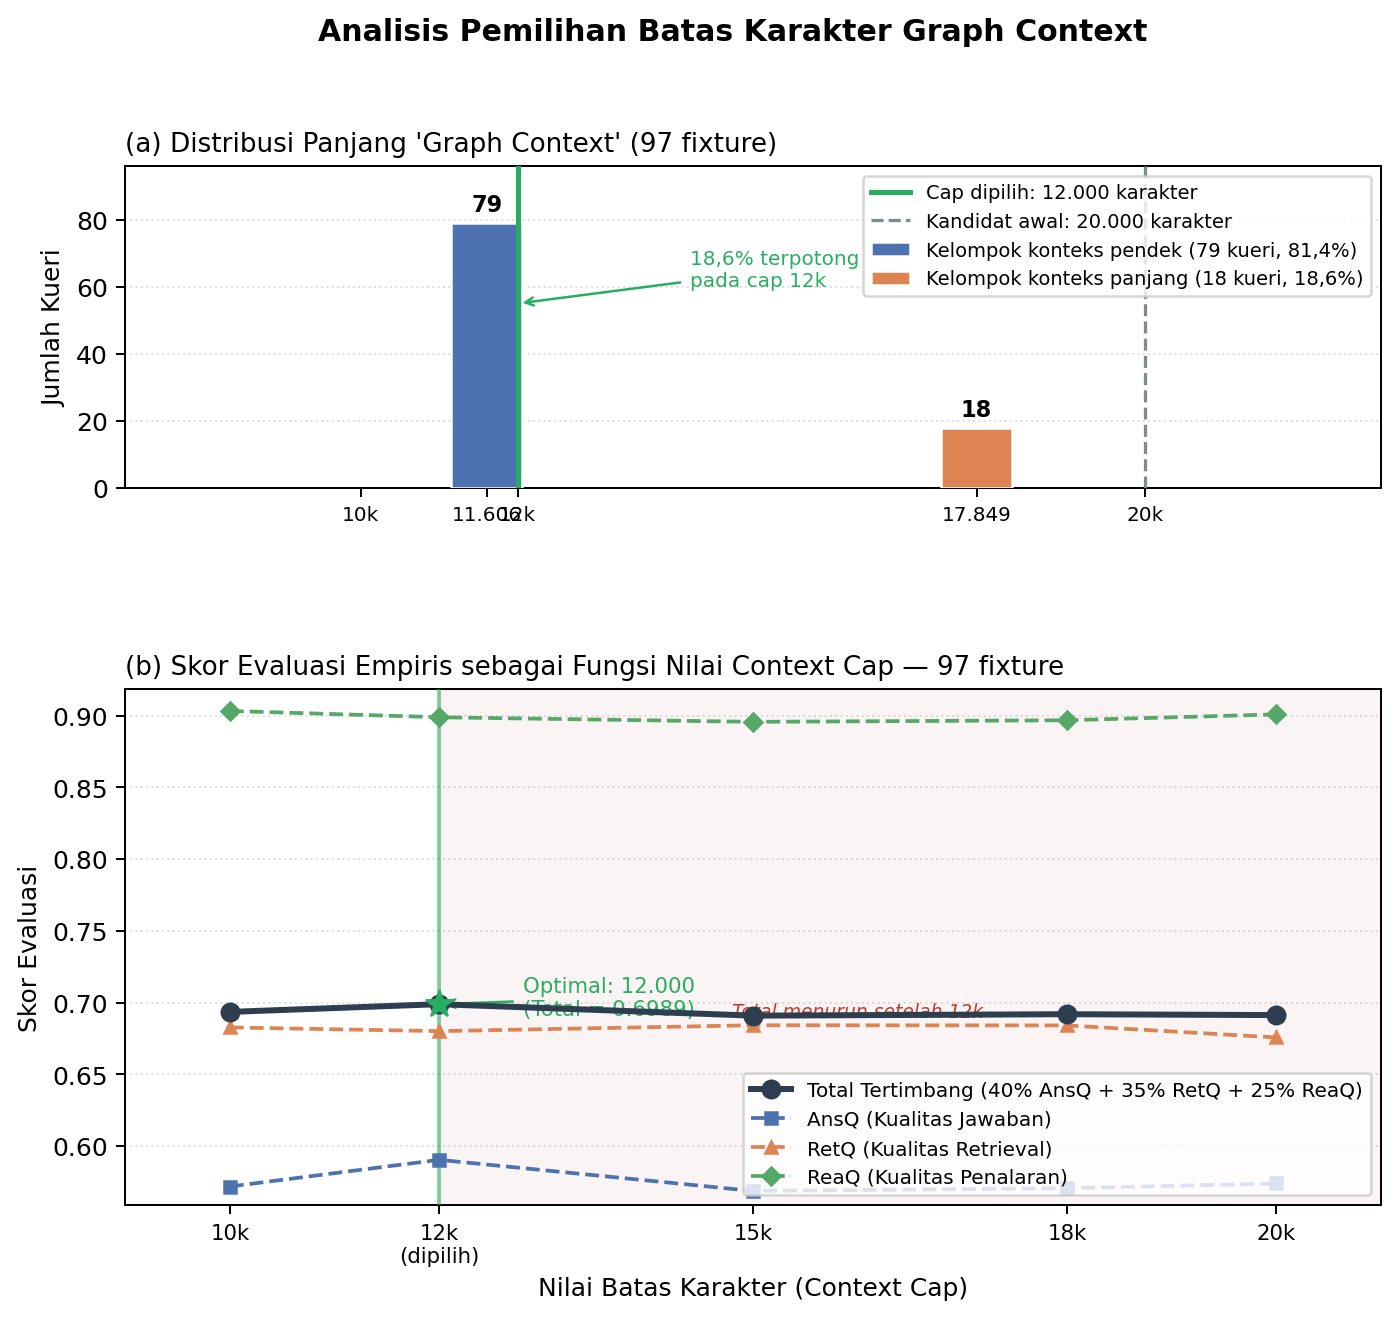
\includegraphics[width=0.88\textwidth]{images/context_cap_selection.png}
    \caption{Analisis pemilihan batas karakter \textit{graph context}. Panel~(a) menunjukkan distribusi bimodal panjang konteks pada 97 \textit{fixture}: 79 kueri (81,4\%) menghasilkan 11.606 karakter dan 18 kueri (18,6\%) menghasilkan 17.849 karakter, dengan garis hijau menandai batas yang dipilih (12.000 karakter). Panel~(b) menunjukkan skor evaluasi empiris (\textit{Total} tertimbang, AnsQ, RetQ, ReaQ) sebagai fungsi nilai batas untuk lima kandidat yang diuji. Batas 12.000 karakter mencapai \textit{Total} tertinggi (0,6989) dan ditetapkan sebagai nilai operasional.}
    \label{fig:context_cap_selection}
\end{figure}

% --- 5.3.2 ---
\subsection{Implementasi Mekanisme \textit{Retrieval} Bertingkat}

Mekanisme \textit{retrieval} diimplementasikan dalam kelas \textit{Stateful\-K8s\-Retriever} pada berkas \texttt{src/chatbot/custom\_retriever.py}. \textit{Method} utama \texttt{retrieve\_context()} menerima parameter \texttt{intent\_data} (hasil ekstraksi Thinker), \texttt{intent\_type} (string jenis \textit{intent}), dan \texttt{max\_depth} (opsional) untuk menghasilkan pasangan \texttt{(graph \_context\_json, reasoning\_path)}.

Pemetaan kedalaman berbasis \textit{intent} diimplementasikan sebagai kamus \texttt{\_DEPTH\_BY\_INTENT} di tingkat modul sebagaimana ditunjukkan pada Listing~\ref{lst:depth-by-intent}. Prioritas resolusi kedalaman adalah: (1) argumen \texttt{max\_depth} yang diberikan secara eksplisit, (2) nilai dari \texttt{\_DEPTH\_BY\_INTENT} berdasarkan \texttt{intent\_type}, dan (3) nilai \textit{default} tiga lompatan. Pemetaan nilai kedalaman untuk setiap tipe \textit{intent} beserta alasan penetapannya ditunjukkan pada Tabel~\ref{tbl:intent_depth_iv}.

\renewcommand{\arraystretch}{1.3}
\captionsetup[table]{justification=raggedright,singlelinecheck=false}
\begin{table}[H]
\caption{Pemetaan \textit{Intent Type} terhadap Kedalaman Traversal Graf}
\label{tbl:intent_depth_iv}
\centering
\begin{tabular}{|p{0.22\textwidth}|p{0.10\textwidth}|p{0.55\textwidth}|}
\hline
\textbf{\textit{Intent Type}} & \textbf{Depth} & \textbf{Alasan} \\
\hline
\texttt{explain} & 2 & Cukup untuk menjawab definisi dan cara kerja \textit{resource}; depth 3+ menambahkan \textit{noise} generik. \\
\hline
\texttt{followup} & 2 & Pertanyaan lanjutan biasanya merujuk entitas yang sama; konteks depth 2 sudah tersedia dari giliran sebelumnya. \\
\hline
\texttt{generate\_yaml} & 3 & Pembuatan YAML membutuhkan field tingkat kontainer (\texttt{image}, \texttt{ports}, \texttt{env}) yang berada di depth 3. \\
\hline
\texttt{trace\_relationship} & 3 & Penelusuran relasi antar-\textit{resource} menjangkau jembatan lintas-\textit{resource} pada depth 2--3. \\
\hline
\end{tabular}
\end{table}


\begin{lstlisting}[language=Python, caption={Kamus kedalaman \textit{traversal} per tipe \textit{intent} (\texttt{\_DEPTH\_BY\_INTENT})}, label={lst:depth-by-intent}]
_DEPTH_BY_INTENT = {
    "explain":            2,
    "followup":           2,
    "generate_yaml":      3,
    "trace_relationship": 3,
    "planning":           3,
}
_DEFAULT_DEPTH = 3  # fallback untuk intent yang tidak dikenali
\end{lstlisting}


Pemilihan nilai kedalaman per tipe \textit{intent} divalidasi secara empiris dengan mengevaluasi seluruh 97 \textit{fixture} pada lima konfigurasi kedalaman tetap ($d \in \{1, 2, 3, 4, 5\}$) dan membandingkan hasilnya terhadap sistem \textit{adaptive}. Gambar~\ref{fig:depth_sensitivity_retq} menunjukkan pengaruh kedalaman traversal terhadap skor RetQ untuk setiap kategori \textit{fixture}, sedangkan Gambar~\ref{fig:depth_sensitivity_submetrics} menunjukkan tren \textit{Precision@k}, \textit{Recall@k}, dan NDCG@k secara agregat.

\begin{figure}[H]
    \centering
    \captionsetup{justification=centering}
    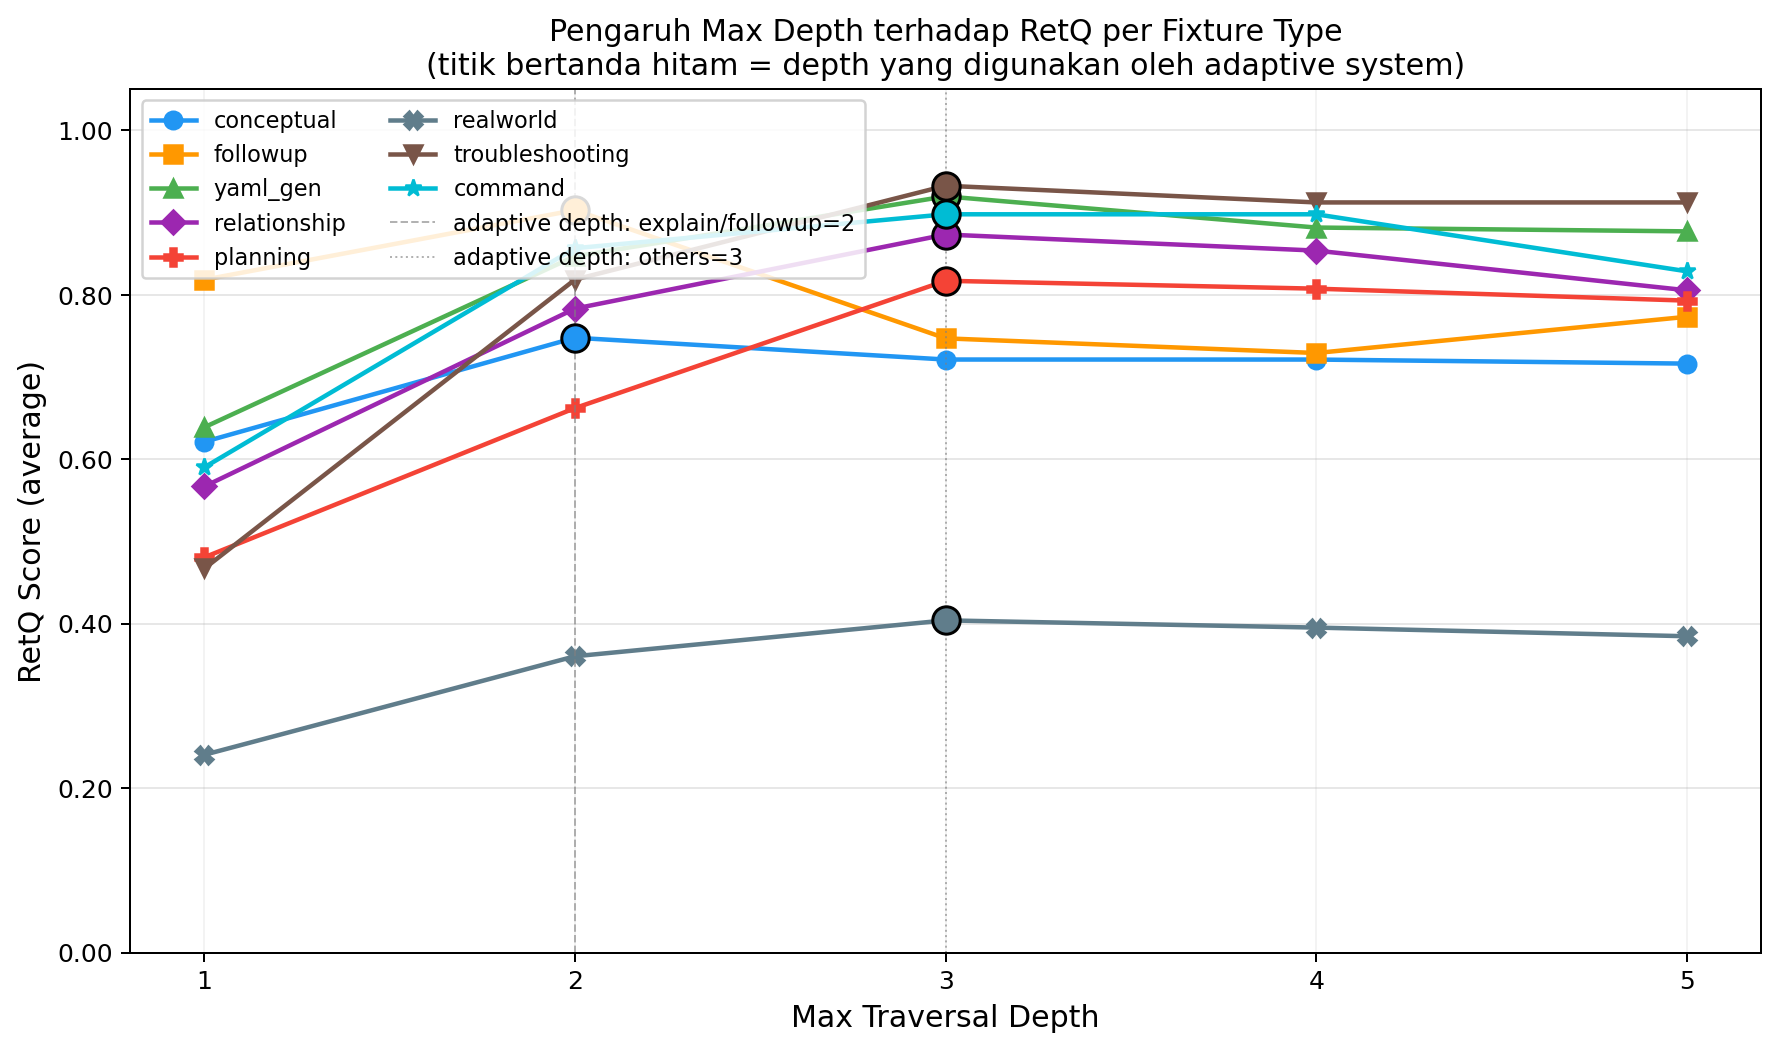
\includegraphics[width=1.00\textwidth]{images/depth_sensitivity_retq.png}
    \caption{Pengaruh kedalaman traversal terhadap RetQ per kategori \textit{fixture}. Titik bertanda hitam menunjukkan kedalaman yang digunakan oleh sistem \textit{adaptive}. Garis putus-putus vertikal menandai kedalaman 2 (\textit{explain}/\textit{followup}) dan kedalaman 3 (kategori lainnya).}
    \label{fig:depth_sensitivity_retq}
\end{figure}

\begin{figure}[H]
    \centering
    \captionsetup{justification=centering}
    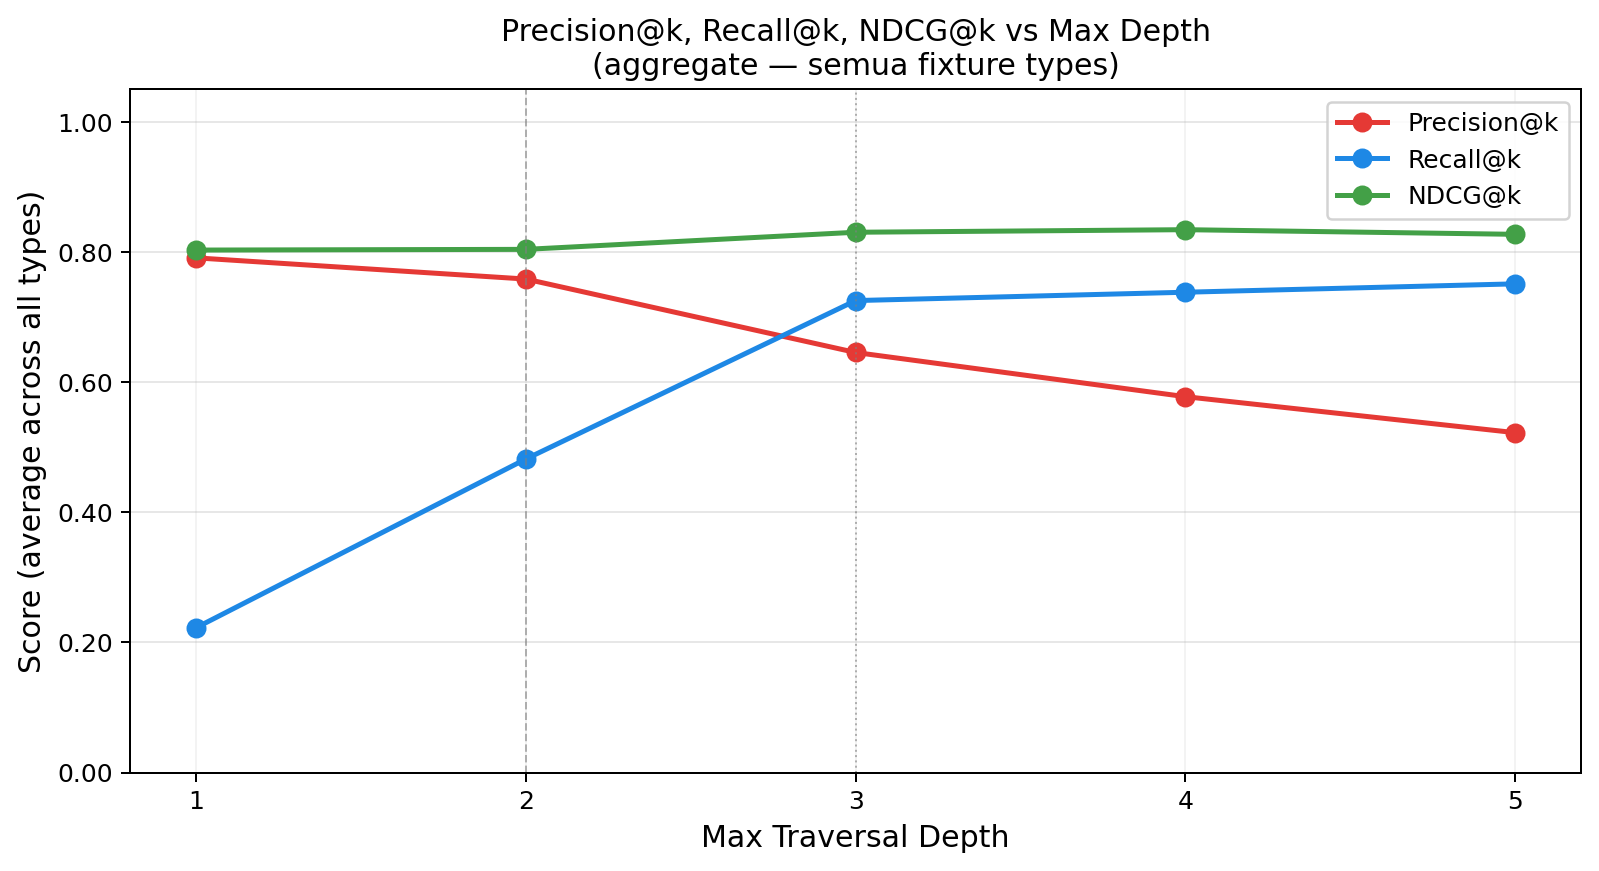
\includegraphics[width=1.00\textwidth]{images/depth_sensitivity_submetrics.png}
    \caption{\textit{Precision@k}, \textit{Recall@k}, dan NDCG@k sebagai fungsi kedalaman traversal (agregat seluruh kategori \textit{fixture}). Nilai optimal terpusat pada kedalaman 2--3, setelah itu skor stabil atau menurun akibat masuknya \textit{node} generik pada kedalaman 4 ke atas.}
    \label{fig:depth_sensitivity_submetrics}
\end{figure}

Pada Fase 1, sistem mengeksekusi \texttt{EXACT\_MATCH\_QUERY} ke Neo4j menggunakan nama sumber daya yang diekstraksi oleh Thinker. Apabila ditemukan, node yang cocok digunakan sebagai \textit{seed node} untuk traversal via \texttt{SCHEMA\_DEPS\_QUERY}. Pada Fase 2—yang hanya diaktifkan jika Fase 1 tidak menghasilkan kecocokan—sistem menghasilkan \textit{embedding} dari kueri menggunakan \textit{text-embedding-3-small} dan mengeksekusi \texttt{HYBRID\_VECTOR\_GRAPH\_QUERY}, yaitu query Cypher tunggal yang menggabungkan \textit{vector similarity search} dengan ekspansi graf di Neo4j. String yang di-\textit{embed} merupakan konkatenasi dari \textit{primary\_resource}, seluruh elemen \textit{related\_concepts}, dan kata kunci ``Kubernetes'', sehingga kemiripan semantik yang dicari mencakup konteks multi-sumber daya secara implisit. Apabila Fase 2 juga tidak menghasilkan kecocokan, \textit{method} mengembalikan pesan \textit{fallback} tanpa melanjutkan traversal.

Untuk \textit{intent} yang melibatkan lebih dari satu sumber daya, yaitu \textit{planning}, \textit{trace\_relationship}, dan \textit{generate\_yaml}, implementasi menambahkan \textit{loop} tambahan yang mengambil konteks dari hingga dua \textit{related\_concepts} yang diekstraksi Thinker dan menggabungkan hasilnya, baik \textit{graph\_context} maupun \textit{reasoning\_path}, dengan hasil dari \textit{primary\_resource}. Penanganan ini diperlukan karena pertanyaan relasional dan generasi YAML multi-komponen membutuhkan konteks skema dari seluruh entitas yang disebutkan, bukan hanya entitas utama. Deduplikasi diterapkan pada \textit{reasoning\_path} agar langkah traversal yang identik antarsumber daya tidak dicatat lebih dari satu kali.

\textit{Reasoning path} dibangun oleh \textit{method} \texttt{\_build\_reasoning\_path()} melalui eksekusi \texttt{PATH\_EDGES\_QUERY} yang menghasilkan daftar \textit{string} berformat \texttt{"Parent -{[}REL{]}-> Child"}, merepresentasikan jalur traversal yang sesungguhnya dari graf, bukan pintasan langsung dari \textit{root} ke \textit{leaf}. Alur keseluruhan mekanisme \textit{cascading retrieval} ini diilustrasikan pada Gambar~\ref{fig:cascading-retrieval}.

\begin{figure}[H]
    \centering
    \captionsetup{justification=centering}
    \includegraphics[width=0.85\textwidth]{images/flowchart-cascading-retrieval.png}
    \caption{Alur mekanisme \textit{cascading retrieval} pada \textit{StatefulK8sRetriever}}
    \label{fig:cascading-retrieval}
\end{figure}

% --- 5.3.3 ---
\subsection{Implementasi Validasi YAML Tiga Lapis}
\label{subsec:implementasi-yaml}

Validasi YAML diimplementasikan dalam kelas \textit{YAMLValidator} pada berkas \texttt{src/validation/yaml\_validator.py} dan hanya diaktifkan secara kondisional ketika \texttt{intent\_type} yang diklasifikasikan oleh node \textit{thinker} adalah \textit{generate\_yaml}, sehingga menghindari \textit{overhead} komputasi untuk pertanyaan penjelasan atau relasi.

Tiga lapisan validasi sebagaimana dirancang pada Tabel~\ref{tbl:yaml_validation_iv} diimplementasikan secara berurutan; lapisan berikutnya hanya dieksekusi apabila lapisan sebelumnya berhasil. Lapis pertama memanggil \texttt{yaml.safe\_load()} dari pustaka PyYAML. Lapis kedua menggunakan \texttt{kubernetes-validate} dengan parameter versi Kubernetes 1.29 sebagai referensi skema. Lapis ketiga mengeksekusi \texttt{REQUIRED\_FIELDS\_QUERY} ke Neo4j untuk memverifikasi keberadaan \textit{field} wajib berdasarkan \textit{knowledge graph} yang telah dibangun pada tahap \textit{ingestion}, sebagaimana ditunjukkan pada Listing~\ref{lst:required-fields-query}.

\begin{lstlisting}[language=SQL, caption={Cypher \textit{query} untuk verifikasi \textit{required fields} pada Lapis 3 Validasi YAML}, label={lst:required-fields-query}]
MATCH (d:Definition {name: $kind})
      -[r:HAS_PROPERTY {is_required: true}]->(p)
RETURN p.name AS field_name
\end{lstlisting}


Keluaran validasi berupa objek \textit{YAMLValidationResult} dengan empat \textit{field}: \texttt{valid} (\textit{Boolean}), \texttt{syntax\_errors} (daftar kesalahan sintaksis PyYAML), \texttt{schema\_errors} (daftar pelanggaran skema Kubernetes), dan \texttt{missing\_fields} (daftar \textit{field} wajib yang tidak ditemukan dalam YAML yang digenerate). Ketika salah satu lapisan mendeteksi kegagalan, antarmuka menampilkan peringatan \texttt{Warning: Potential Syntax Error} kepada pengguna.

% ─────────────────────────────────────────────────────────────────────
\section{Implementasi Sistem Pembanding: Vector RAG dan Vanilla LLM}
\label{sec:implementasi-baseline}
% ─────────────────────────────────────────────────────────────────────

Kedua sistem pembanding yang dirancang pada Subbab~\ref{sec:perancangan-baseline} diimplementasikan dalam berkas \texttt{scripts/evaluate.py} sebagai mode eksekusi yang dapat dipilih melalui argumen \texttt{-{}-mode}.

\begin{enumerate}
    \item \textbf{Vanilla LLM} (\texttt{-{}-mode llm}) \\
    Implementasi Vanilla LLM memanggil GPT-4o-mini secara langsung menggunakan \texttt{HumanMessage} yang berisi pertanyaan pengguna tanpa konteks tambahan. Sistem tidak melakukan \textit{retrieval} apapun, sehingga jawaban bergantung sepenuhnya pada pengetahuan parametrik model.

    \item \textbf{Vector RAG} (\texttt{-{}-mode vector}) \\
    Implementasi Vector RAG menggunakan \texttt{VectorIndexManager} untuk menghasilkan \textit{embedding} kueri dengan \textit{text-embedding-3-small}, kemudian mengeksekusi \texttt{SIMPLE\_GRAPH\_EXPAND\_QUERY} ke Neo4j untuk mengambil top-$k$=5 \textit{node} terdekat beserta satu lompatan ekspansi ke \textit{node} tetangga. Konteks yang dihasilkan diteruskan ke \textit{speaker} GPT-4o-mini. Sistem ini tidak menggunakan \textit{intent-adaptive depth traversal} maupun validasi YAML.
\end{enumerate}

Hasil evaluasi komparatif ketiga sistem disajikan pada Bab~\ref{chap:evaluasi}.

